\documentclass[12pt]{article}

\usepackage[letterpaper,margin=1in]{geometry}

\setlength{\parindent}{0pt}

\usepackage{amssymb}
\usepackage{amsmath}

\usepackage{multicol}

\usepackage{tikz}

\newcommand{\headerText}{
  MA 238 | Fall 2018 | Dr. Clontz
}

\usepackage{fancyhdr}
\pagestyle{fancy}
\renewcommand{\headrulewidth}{0pt}% Default \headrulewidth is 0.4pt
\renewcommand{\footrulewidth}{0pt}% Default \footrulewidth is 0pt
\chead{\footnotesize\bf\headerText}
\cfoot{}

\newcommand{\csch}{\operatorname{csch}}
\newcommand{\sech}{\operatorname{sech}}

\newcommand{\issuesMark}{{\fontencoding{U}\fontfamily{futs}\selectfont\char 66\relax}}

\newcommand{\response}{
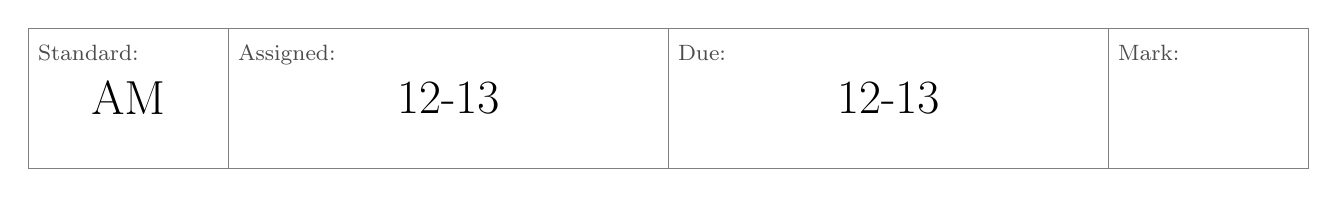
\begin{tikzpicture}[x=1in,y=0.7in]
  \draw[color=black!50] (0,0) rectangle (6.4,1);
  \draw[color=black!50] (1,0) -- (1,1);
  \draw[color=black!50] (3.2,0) -- (3.2,1);
  \draw[color=black!50] (5.4,0) -- (5.4,1);

  \node[anchor=north west,color=black!70] at (0,0.95) {\footnotesize Standard:};
  \node at (0.5,0.5) {\LARGE AM};
  \node[anchor=north west,color=black!70] at (1,0.95) {\footnotesize Assigned:};
  \node at (2.1,0.5) {\LARGE 12-13};
  \node[anchor=north west,color=black!70] at (3.2,0.95) {\footnotesize Due:};
  \node at (4.3,0.5) {\LARGE 12-13};
  \node[anchor=north west,color=black!70] at (5.4,0.95) {\footnotesize Mark:};
\end{tikzpicture}
}


\begin{document}

\begin{center}
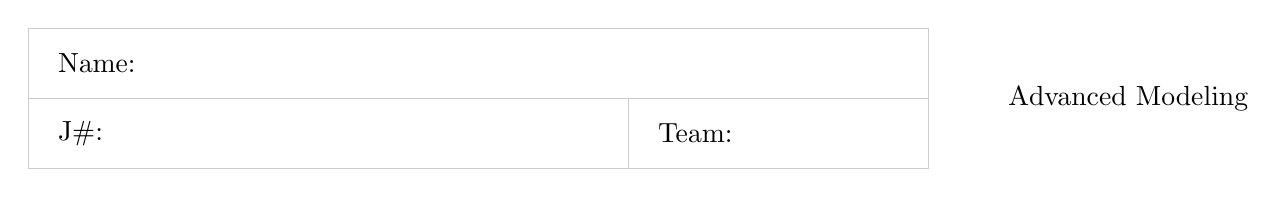
\begin{tikzpicture}[x=1in,y=0.7in]
  \draw[color=black!20] (0,0) rectangle (4.5,1);
  \draw[color=black!20] (0,0.5) -- (4.5,0.5);
  \draw[color=black!20] (3,0) -- (3,0.5);

  \node[anchor=west] at (0.1,0.75) {Name:};
  \node[anchor=west] at (0.1,0.25) {J\#:};
  \node[anchor=west] at (3.1,0.25) {Team:};

  \node at (5.5,0.5) {Advanced Modeling};
\end{tikzpicture}
\end{center}

\vspace{1em}

\response

A certain rocket's velocity is modeled by the following IVP:

\[
2500v'=50u(t)-50u(t-40)
\hspace{1em}
v(0)=20
\]

What will the velocity of the rocket be after \(100\) seconds?

\end{document}
